\chapter{Scalable Distributed Systems}

\paragraph{
HPC and mainframes.
}
\begin{itemize}
\item Pros: Single solution, powerful hardware, reliable design
\item Cons: £££, failure models, vendor lock-in, adaptability
\end{itemize}

\paragraph{Distributed Computing.} Want to achieve linear scalability, but
synchronization, communication (\textbf{overheads}) prevent it. Ideally, perfect
partition of data and compute (e.g. distribute client/server model on
\textbf{cheap commodity hardware} (best £/resource) and account for failures and
manage the network speed bottleneck in software (parallel algorithms and
systems).

\paragraph{Data centers} Usually DC will have non-commodity network, but it will
still the slowest part in memory hierarchy. Focus on \textbf{scaling-out} not up
by buying cheap hardware in bulk therefore achieve economy of scale. Elasticity:
Resources on-demand (illusion of infinite resource).

\section{Properties of DS}
\begin{itemize}
\item Scalability: By aggregation of many resources
  \begin{itemize}
  \item Compute
  \item Storage: distributed file systems
  \item Memory: cluster memory (in-memory key/value stores, caches)
  \item Bandwidth: DC networks, CDN
  \end{itemize}
  \item location transparency from the user's perspective (black box API)
  \item High availability: Mask hardware and software failures
  \item Composition of services
\end{itemize}
\subsection{Answering a google search request}
\begin{enumerate}
\item Load-balancer routes request to lightly-loaded Google Web Server (GWS)
\item GWS routes search to one Index Server for each shard through load-balancer
\item Results are aggregated (IDs for matching documents), ie ordered by
  relevance
\item GWS sends appropriate IDs to Doc Servers to retrieve URL, title, summary
\item Results are aggregated (+ad, spell), producing search result page
\end{enumerate}

\section{Design principles}
\paragraph{Types of scalable systems}
\begin{enumerate}
\item Online systems ($<$100 ms) (OLTP)
\item Batch processing systems ($>$1 hours) (OLAP)
\item Nearline systems ($<$1 secs or mins)
\end{enumerate}

\paragraph{Distributed Computing Challenges}
\begin{itemize}
\item \textbf{Scalability}: Independent parallel processing of
  sub-requests/tasks. More servers permits serving more concurrent requests.
\item \textbf{Fault tolerance}: Mask and recover from HW/SW failure. Replication
  data and service.
\item \textbf{High availability}
\item \textbf{Consistency}: $/neq$ services but $=$ results.
\item \textbf{Performance}: \textbf{Predictable} low-latency processing with
  high throughput
\end{itemize}

\paragraph{Abstractions}: Each layer should be itself scalable.\\
    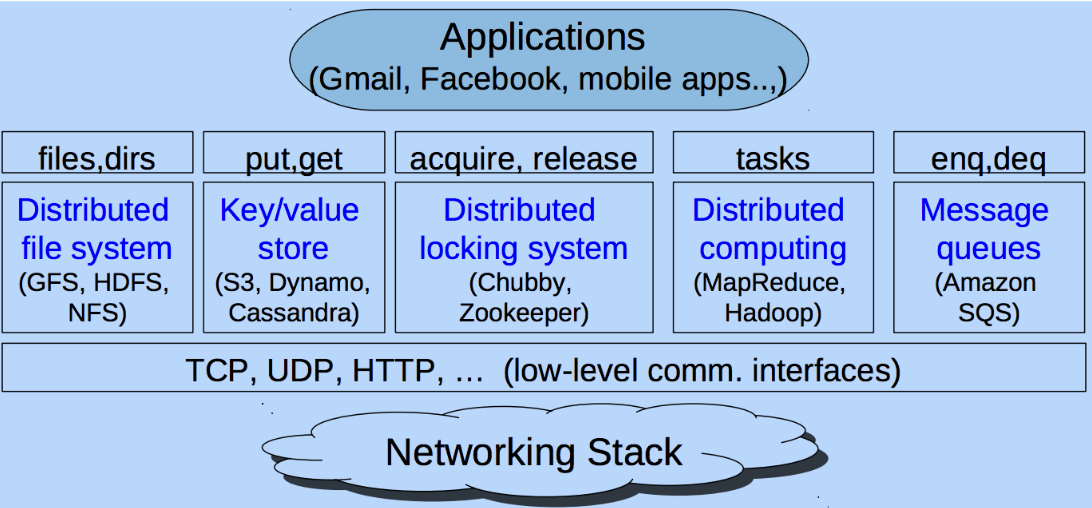
\includegraphics[width=0.59\textwidth]{img/abstraction.png}\\
%\begin{wrapfigure}{R}{0.6\textwidth}
%\end{wrapfigure}\\

\paragraph{Design principles}
\begin{itemize}
\item \textbf{Stateless services}: Avoid data inconsistency. Separation of data +
  meta-data, Use lease.
\item \textbf{Caching}: Latency.
\item \textbf{Partition/aggregration pattern} (see google search above)
\item \textbf{Consistency models}: (Most apps use a mix of strong and others).
  Switch to weaker for latency reasons. Decide what matters (e.g. Order of posts
  in LinkedIn news feed? Access from multiple devices?)
\item \textbf{Efficient failure recovery}: Failure is very common, but full redundancy
  too expensive $\rightarrow$ failure recovery $\Rightarrow$ Rather reduce the cost of failure recovery.
  \begin{itemize}
    \item Replication: Need to replicate data and service (consistency issues)
      \item Recomputation: Use stateless protocols, form data lineage for compute jobs
  \end{itemize}
\end{itemize}